\documentclass{standalone}
\usepackage{tikz}
\begin{document}
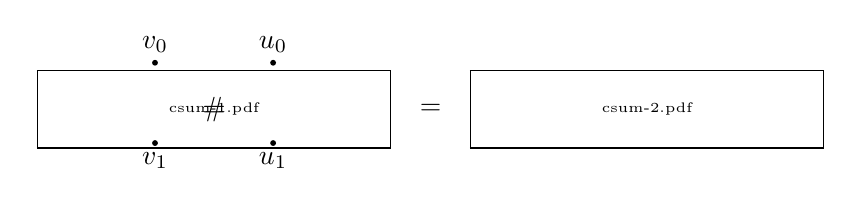
\begin{tikzpicture}
  \pgfdeclareimage[width=4.5cm]{lhs}{csum-1.pdf}
  \pgfdeclareimage[width=4.5cm]{rhs}{csum-2.pdf}
  \node () at (-2.75, -2.75) {$\#$};
  \node () at (0, -2.75) {$=$};
  % \draw[|-latex] (-1, -1.5) -- (1, -1.5);
  \node () at (-2.75,-2.75) {\pgfuseimage{lhs}};
  \node () at (2.75,-2.75) {\pgfuseimage{rhs}};

  \begin{scope}[every node/.style={fill=black, circle, inner sep=.75pt}]
    \node (a) at (-3.5, -2.16) {};
    \node (b) at (-3.5, -3.18) {};
    \node (c) at (-2, -2.16) {};
    \node (d) at (-2, -3.18) {};
  \end{scope}


  \node[above] () at (a) {$v_0$};
  \node[below] () at (b) {$v_1$};
  \node[above] () at (c) {$u_0$};
  \node[below] () at (d) {$u_1$};


\end{tikzpicture}
\end{document}
